\chapter{Implementation}
\thispagestyle{main} % Needed for Footer and Header on Chapterpage
This chapter focuses on explaining why things were implemented in a certain manner. In this chapter the trade-offs and decisions which were made while building the VM are described in a manner that follow up works get a better understanding of why some parts of the VM are implemented in a certain way so that they either are more certain when changing something or to help them reach the same conclusion faster.

\section{Software Architecture}
Figure \ref{package overview} shows the structure of the project on package-level and the dependencies among them. The miner application was built with software engineering principles in mind. Particular attention was paid to modularity. This made it easy to integrate the virtual machine into the existing miner application. Furthermore the following figure shows which packages were added and which where modified to successfully integrate the execution of smart contracts into the Bazo blockchain. As the miner and all other projects are written in Go, the new components are written in Go aswell.
\begin{figure}[H]
	\begin{center}
	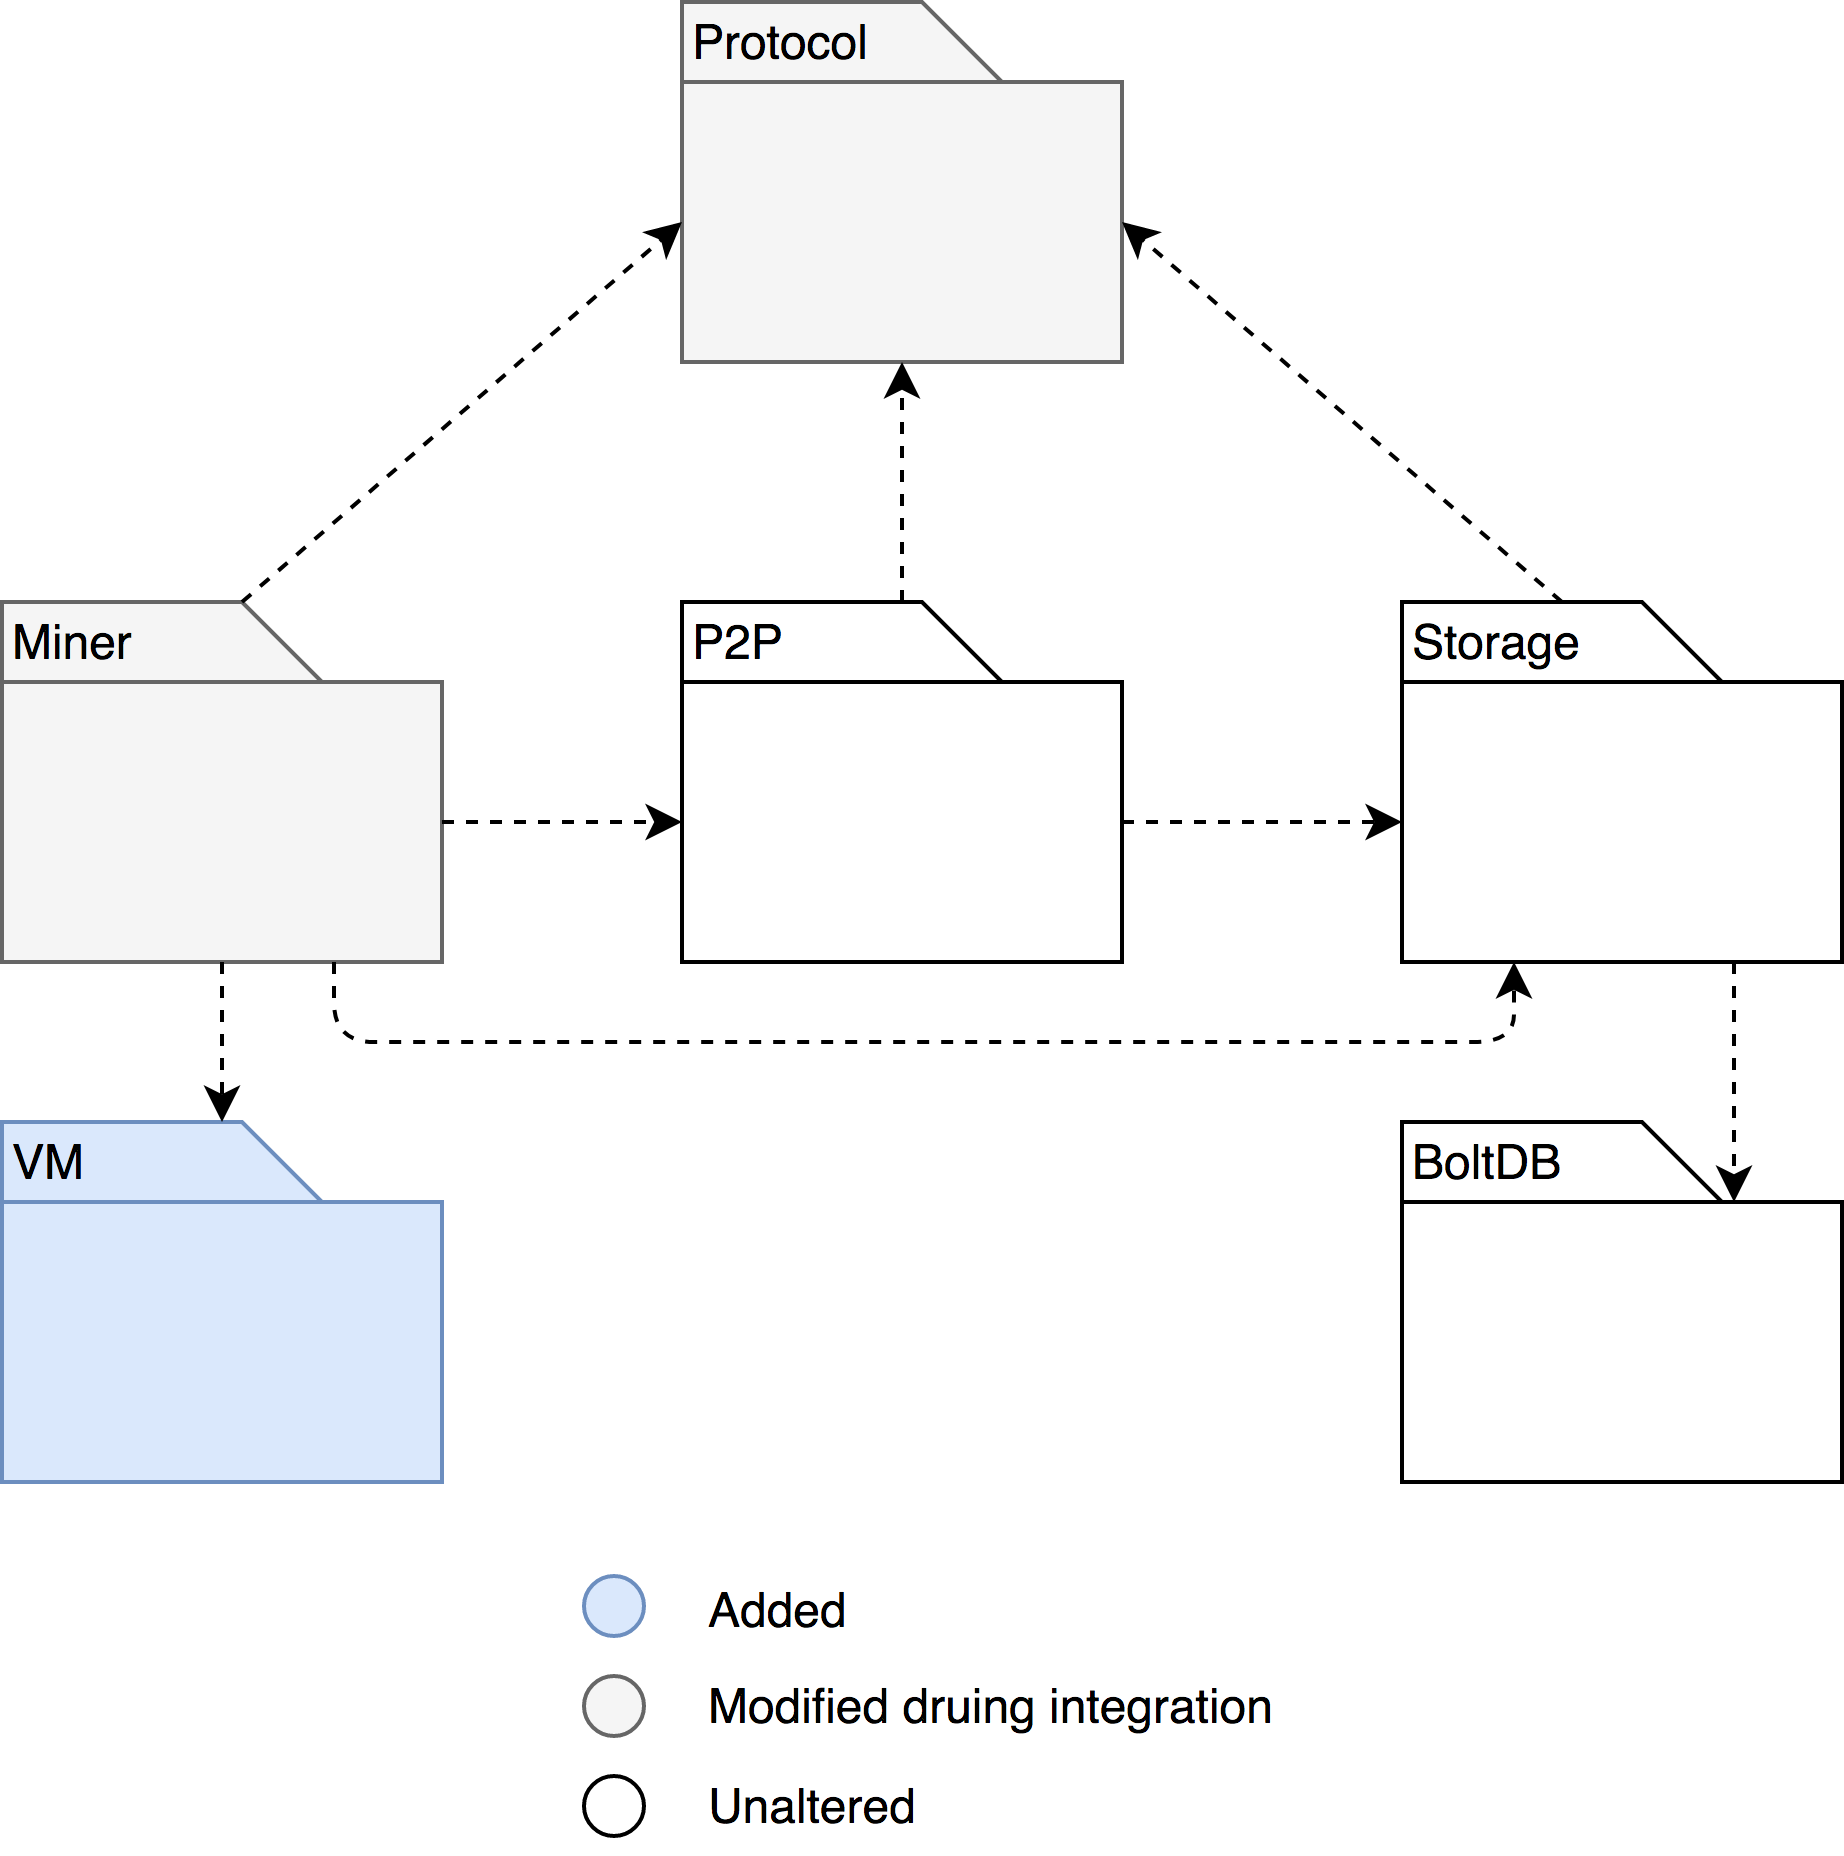
\includegraphics[width=0.8\textwidth]{./images/package-diagram}
	\caption{UML Package Diagram}
	\label{package overview}
	\end{center}
  \end{figure}

\begin{description}
	\item[Protocol] This package contains the building blocks for the Bazo blockchain. In particular it contains the structure, encoding, decoding and hashing functions of all transaction types, blocks and accounts. In addition a transaction interface is defined, allowing an abstract treatment of transactions. \cite{ba_miner}
	\item[Miner] The miner package contains all mining related components. That includes the validation and consolidation of transactions into blocks, the calculation of the consensus mechanism and the building of the merkle tree. In addition to that, blockchain related tasks itself such as rollback operation and state changes are contained in this package. Access to P2P and Storage packages are needed in order to handle transactions over the network and signal storage-related operations. \cite{ba_miner} To execute the virtual machine and access its results, the miner also needs access to the VM package.
	\item[VM] This package contains the virtual machine itself and all its components, namely the evaluation stack, the call stack, implementations of data structures that can be used by the virtual machine such as array and map and all available opcodes.
	\item[P2P] All networking related operations are implemented in the P2P package \cite{ba_miner}. Since for the integration of the virtual machine nothing had to be changed, the content of this package is not discussed any further.
	\item[Storage] The storage package is concerned with memory-related tasks. The lower-level functionality was implemented with the external BoltDB package. Since entries are encoded before writing to storage and decoded when loaded \cite{ba_miner}, this package could be left unaltered. For that reason, this package is also not described further.
	\item[BoltDB] This package shows the BoltDB package which is an external dependency. BoltDB is a simple, lightweight key/value base. \cite{ba_miner}
	\item[Parser] The Parser package contains the parser, which consists of a Tokenize and Parse function and tokens. This components are needed to compile \flqq Enhanced Bazo byte code\frqq{ } to a byte code instruction set that can be interpreted by the virtual machine. This package is completely stand-alone and does not have any dependencies. The package is also kept in a separate repository.
\end{description}

\section{Protocol}
As mentioned in Section \ref{design_miner} the structs of Account, FundsTx and AccTx had to be adapted. The structs originally had a fixed length. The structs are transferred encoded between the individual components, to achieve loose coupling. The original encoding and decoding functions of those structs is based on the fixed length of the struct. Since the added fields are optional and have an arbitrary length, the encoding and decoding functions had to be redesigned. It was decided use the gob package, which is a package from the Go standard library. The gob package manages streams of binary values between an encoder and decoder. A stream of gobs is self-describing. \cite{golang_gob} The main disadvantage is, that these functions no longer are platform independent.

\subsection{Encoding}
The new encoding function for the AccTx struct is shown in figure \ref{new_encode}. Switching to gob has lead to a better readability and to fewer lines of code. The type information is defined in line 2. The function \mintinline{go}{.Encode()} in line 12 makes sure all type information data is sent before it is needed. \cite{golang_gob} The encoding functions of the other structs, that were redesigned are very similar and therefore not dealt with. 

\begin{figure}[thp]%
    	\centering
		\begin{minipage}{0.7\textwidth}
		\begin{minted}
		[
		frame=lines,
		autogobble,
		framesep=2mm,
		baselinestretch=1.2,
		fontsize=\footnotesize,
		linenos
		]{go}
		func (tx *AccTx) Encode() (encodedTx []byte) {
			encodeData := AccTx{
				tx.Header,
				tx.Issuer,
				tx.Fee,
				tx.PubKey,
				tx.Sig,
				tx.Contract,
				tx.ContractVariables,
			}
			buffer := new(bytes.Buffer)
			gob.NewEncoder(buffer).Encode(encodeData)
			return buffer.Bytes()
		}
		\end{minted}
		\caption{New gob based encoding function}
		\label{new_encode}
		\end{minipage}
\end{figure}

\subsection{Decoding}
Figure \ref{new_decode} shows the decoding function of AccTx. The \mintinline{go}{decoder.Decode()} function in line 5 reads the next value from the input stream and stores it in the data represented by the AccTx interface. \cite{golang_gob}

\begin{figure}[thp]%
    	\centering
		\begin{minipage}{0.7\textwidth}
		\begin{minted}
		[
		frame=lines,
		autogobble,
		framesep=2mm,
		baselinestretch=1.2,
		fontsize=\footnotesize,
		linenos
		]{go}
		func (*AccTx) Decode(encodedTx []byte) *AccTx {
			var decoded AccTx
			buffer := bytes.NewBuffer(encodedTx)
			decoder := gob.NewDecoder(buffer)
			decoder.Decode(&decoded)
			return &decoded
		}
		\end{minted}
		\caption{New gob based decoding function}
		\label{new_decode}
		\end{minipage}
\end{figure}

\section{Miner}
\subsection{Constructors}
AccTxs now have an optional field for contracts and contract variables, if it remains a standard AccTx nil has to be passed for both parameters in the constructor. The same applies to the FundsTx. If the transaction is intended to be a regular FundsTx, the data field has to be nil. 

\subsection{VM entry point}
The balance of a FundsTx is updated in the \mintinline{go}{addFundsTx()} in the block.go class. Therefore this function is the ideal entry point for the virtual machine. Figure \ref{addFundsTx} shows the function without parts that are irrelevant for the integration. Before the function checks whether the transaction calls a smart contact, it performs various checks, i.e. if the account exists or if the sender has a balance high enough to transfer the defined amount of Bazo coins. If all this checks are successful the function validates if the transaction is a valid smart contract call. If so, a new context object with the receiver account and the transaction is created as seen in line 8. As next step the virtual machine is initialized with the context object. In line 12 the \mintinline{go}{Exec()} function is called which starts the virtual machine. If the \mintinline{go}{Exec()} function returns with an error the execution of the addFundsTx is aborted and the context changes are not persisted. After the VM execution, the finalizing steps are carried out, such as updating the balances of both accounts and writing the block header to storage.

\begin{figure}[thp]%
    	\centering
		\begin{minipage}{0.8\textwidth}
		\begin{minted}
		[
		frame=lines,
		autogobble,
		framesep=2mm,
		baselinestretch=1.2,
		fontsize=\footnotesize,
		linenos
		]{go}
func addFundsTx(b *protocol.Block, tx *protocol.FundsTx) error {
	... // Various checks
	// Check if transaction has data and the receiver account 
	// has a smart contract
	if tx.Data != nil && b.StateCopy[tx.To].Contract != nil {
		context := protocol.NewContext(*b.StateCopy[tx.To], *tx)
		virtualMachine := vm.NewVM(context)

		// Check if vm execution run without error
		if !virtualMachine.Exec(false) {
			return errors.New(virtualMachine.GetErrorMsg())
		}
		
		//Update changes vm has made to the contract variables
		context.PersistChanges()
	}
	... // Finalization
}
		\end{minted}
		\caption{addFundsTx function}
		\label{addFundsTx}
		\end{minipage}
\end{figure}

% \subsection{Adjustment of Transaction Encoding}

% \subsection{Adjustment of opcodes to context and miner}

\section{Virtual Machine}

At the time of writing this thesis the VM consists of the following classes:
% Insert execution cycle graphic

\subsection{Stack}

% TODO insert crc card for stack

\subsubsection{Maximum stack size}
Facing the concern of excess memory usage of the contract on the miner, we decided to limit the stack size to 1MB which seems to be well above what the contracts will need. We neglected using the gas amount for max storage determination because it would be just a soft limit

\subsubsection{Maximum variable size}
Since it is possible to easily craft denial of service attacks for the blockchain if there is no limit on the variable size we decided to set the variable size to a specific fixed amount instead of arbitrary precision.

\subsubsection{Data structure}
As underlying data structure of "Stack", keeping in mind to keep the code of the vm short and simple, we decided to use an array of big.Int. It was important that the datatype used for the underlying datatype was of arbitrary length because splitting up an element into multiple bytes so that it can be saved when using an array of bytes as underlying data structure would have been a lot more complex and more error-prone. Arbitrary length is implemented for example an array of jagged arrays of bytes. On the vm it was very important that the type used in the vm provided mathematical methods and also that it could store and work with values of up to 256 bit size. Only big.Int fulfilled both requirements and therefore it was choosen for the vm. Thanks to big.Int being of arbitrary length we could then use an array of big.Int as underlying data structure which also simplifies our code since we don't have to cast the values retrieved from the stack before working with them.

We neglected working with pointers because even though there are more elements created on the heap of the physical machine, it shouldn't make a difference considering the vast availability of resources on modern computers and our rather small contracts. We neglected using a simple array of bytes as the whole data structure where different datatypes are read using a different amount of bytes, as it is common when having no abstraction layer or using a jagged array of byte arrays because the could becomes a lot more readable in the vm and less conversions from big.Int to byte array are necessary. We accept the dependency on the datatype big.Int which is necessary as it implements all mathematical operations which are very important and because it is of arbitrary precision and the size of other datatypes would not have been sufficient especially for cryptographic purposes.
% \subsection{Contract Execution}

\subsection{Virtual machine}

\subsubsection{Exec() function}
The main part of the virtual machine itself is the \mintinline{go}{Exec()} function which contains the execution cycle of the virtual machine as mentioned in section \ref{exec_cycle}. 


% TODO insert crc card for vm
\subsubsection{opCodes}
% Please add the following required packages to your document preamble:
% \usepackage{booktabs}
\begin{table}[]
\centering
\caption{List of opCodes available}
\label{opcodes cheat sheet}
\begin{tabular}{@{}llll@{}}
\toprule
\textbf{Instruction} & \textbf{Mnemonic} & \textbf{opCode} & \textbf{Description}                                     \\ \midrule
Push Bytes           & PUSH              & 0x00            & stack $\leftarrow$ bytes                                            \\
Duplicate            & DUP               & 0x01            & stack $\leftarrow$ peek1                           \\
Roll                 & ROLL              & 0x02            & removes element at index and push to ToS           \\
Pop                  & POP               & 0x03            & pops ToS                                                 \\
Add                  & ADD               & 0x04            & stack $\leftarrow$ pop1 \+ pop2                                      \\
Subtract             & SUB               & 0x05            & stack $\leftarrow$ pop1 \- pop2                                      \\
Multiply             & MULT              & 0x06            & stack $\leftarrow$ pop1 \* pop2                                      \\
Divide               & DIV               & 0x07            & stack $\leftarrow$ pop1 \/ pop2                                      \\
Modulo               & MOD               & 0x08            & stack $\leftarrow$ pop1 \% pop2                                     \\
Negate               & NEG               & 0x09            & stack $\leftarrow$ todo                                             \\
Equals               & EQ                & 0x0a            & stack $\leftarrow$ 1 if pop1 == pop2, 0 otherwise                   \\
Not equal            & NEQ               & 0x0b            & stack $\leftarrow$ 1 if pop1 != pop2, 0 otherwise                   \\
Lower than           & LT                & 0x0c            & stack $\leftarrow$ 1 if pop1 \textless{} pop2, 0 otherwise            \\
Greater than         & GT                & 0x0d            & stack $\leftarrow$ 1 if pop1 \textgreater{} pop2, 0 otherwise         \\
Lower than/equals    & LTE               & 0x0e            & stack $\leftarrow$ 1 if pop1 \textless{}= pop2, 0 otherwise         \\
Greater than/equals  & GTE               & 0x0f            & stack $\leftarrow$ 1 if pop1 \textgreater{}= pop2, 0 otherwise      \\
Shift left           & SHIFTL            & 0x10            & stack $\leftarrow$ pop 1 \textless{}\textless nrOfShifts            \\
Shift right          & SHIFTR            & 0x11            & stack $\leftarrow$ pop 1 \textgreater{}\textgreater nrOfShifts      \\
No operation         & NOP               & 0x12            & does nothing                                             \\
Jump                 & JMP               & 0x13            & jump to address                                          \\
Jump if true         & JMPIF             & 0x14            & jumps to address if pop1 == 1                            \\
Call                 & CALL              & 0x15            & call a function                                          \\
Call if true         & CALLIF            & 0x16            & calls a function if pop1 == 1                            \\
Call external        & CALLEXT           & 0x17            & calls function from external smart contract              \\
Return               & RET               & 0x18            & returns from function                                    \\
Size of ToS          & SIZE              & 0x19            & stack $\leftarrow$ size(pop1)                                       \\
Store                & STORE             & 0x1a            & stores pop1 in callStack                                 \\
State Store          & SSTORE            & 0x1b            & stores pop1 in contractVariables                         \\
Load                 & LOAD              & 0x1c            & stack $\leftarrow$ var from callStack
    \\
State Load           & SLOAD             & 0x1d            & stack $\leftarrow$ receiver var from contractVariables \\
Address              & ADDRESS           & 0x1e            & stack $\leftarrow$ receiver account address                         \\
Balance              & BALANCE           & 0x1f            & stack $\leftarrow$ receiver account balance                         \\
Caller               & CALLER            & 0x20            & stack $\leftarrow$ contract caller                                  \\
Call value           & CALLVAL           & 0x21            & stack $\leftarrow$ transaction amount in bazo coins                 \\
Call data            & CALLDATA          & 0x22            & stack $\leftarrow$ transaction data                                 \\
New map              & NEWMAP            & 0x23            & stack $\leftarrow$ new map                                          \\
Map push             & MAPPUSH           & 0x24            & stack $\leftarrow$ add entry to map                                 \\
Map get value        & MAPGETVAL         & 0x25            & todo                                                     \\
Map set value        & MAPSETVAL         & 0x26            & todo                                                     \\
Map remove           & MAPREMOVE         & 0x27            & todo                                                     \\
New array            & NEWARR            & 0x28            & stack $\leftarrow$ new array                                        \\
Array append         & ARRAPPEND         & 0x29            & todo                                                     \\
Array insert         & ARRINSERT         & 0x2a            & todo                                                     \\
Array remove         & ARRREMOVE         & 0x2b            & todo                                                     \\
Array index at       & ARRAT             & 0x2c            & todo                                                     \\
SHA3 Hashing         & SHA3              & 0x2d            & stack $\leftarrow$ SHA3\_HASH(pop 1)                                \\
Check signature      & CHECKSIG          & 0x2e            & todo                                                     \\
Halt with error      & ERRHALT           & 0x2f            & return from Exec() function with false                   \\
Halt                 & HALT              & 0x30            & return from Exec() function with true                    \\ \bottomrule
\end{tabular}
\end{table}

\subsubsection{Arithmetic}
The arithmetic opcodes are based on the arithmetic operations provided by big.Int. The two elements on top of the stack are popped, the arithmetic operation is executed and the result is pushed back to the stack. It is not necessary to take care of casting different int types such as uint32 to uint64 if the result is bigger than the two operands, since that is done by big.Int.

\subsubsection{Bit operations}
Two opcodes for shifting bits to the right and the left. Same as arithmetic, this is based on the implementation of big.int.

\subsubsection{Controlflowoperations}


\subsubsection{Datastructures}
The datastructures the vm can create are map, array and struct on top of an array. 

\begin{tabular}[t]{ p{3cm} p{12.5cm}}
\textbf{NEWMAP} & 
The opcode NEWMAP creates a new map and pushes it on the stack. 
\\ \\

\textbf{MAPPUSH} & 
\\ \\

\textbf{MAPGETVAL} & 
\\ \\

\end{tabular}

The two basic datastructures map and array are directly implemented as opcodes

describe the implementation of map, array and how one could create a struct. Do it the same as the other opcodes.

\begin{tabular}[t]{ | c | c | c | c | }
\textbf{opcode} &
\textbf{Description} &
\textbf{Input} &
\textbf{Output} \\ \hline

NEWMAP &
Creates a new map and pushes it on the stack. &
- &
map \\ \hline

MAPCONTAINSKEY &
Consumes a map and pushes true or false on the stack depending on wether the map contained the key. &
map &
bool \\ \hline

\end{tabular}

\subsection{Context}
For the vm execution to have any effect it is necessary to change the state of the miner eventually. The problem with an immediate change of the miner state is that the contract execution could fail in the middle of the contract resulting in inconsistencies. Such inconsistencies could be resolved with rollback but since this is rather difficult to implement because something keeping track of the changed data, it was decided to provide the state as a copy in a context object. The VM would later on perform the changes to contract data. The changed contract data would later on be written back by the miner after a successfull contract execution


This was implemented using an interface because all the methods the VM can use are easily readable in the interface 

which made it possible to create a special context mock type for testing and one for the actual miner implementation. This was and is useful when having to redefine methods, it also makes it more clear to what the vm actually has acces via reading the context interface. 


Since the state of the vm is not persisted 

The context describes all variables outside the 

\subsection{Sideffects on data}

Since the VM operates on copies the values will also not be changed by a faulty contract.

\subsection{Error handling}
Since the virtual machine just processes one instruction set after another and the smart contracts have to be written directly in these opcodes it is easily possible to write byte code which is not possible for the vm to execute, for example byte code which tells the vm to push six bytes on the stack when there is only one byte left in the instruction set. This of course means that an error occurs somewhere in the vm which could terminate the miner. This should neither be possible by accident nor by choice.

Therefore it was paid a lot of attention to put guards around functions possibly throwing an error to avoid calling accordant functions with invalid values and define graceful failures with an error object. The message of this error object is later on pushed on the stack of the vm after that the vm halts. Also to make the debugging less complicated, the name of the opcode in which the error occoured is added to the front of the error code, therefore it is possible to determine what caused the error up to instruction kind.

\section{Parser}
The language the parser processes cannot be described as a high-level programming language and is very strongly aligned to the actual byte code, which is why the parser is very basic. The parser package contains two classes and a test file. One class is tokens.go, which contains the available opcodes with its arguments, and the token types. The second class is parser.go, which can be split into two main functions. 

\subsection{Tokens class}
\begin{tabular}[t]{ p{3cm} p{12.5cm}}
\raggedright
\textbf{Token struct and types} &
Code snippet \ref{tokenstruct} shows the Token struct. The tokenType field can be \mintinline{go}{OPCODE} (Value: 0), \mintinline{go}{INT} (Value: 1), \mintinline{go}{BYTE} (Value: 2), \mintinline{go}{BYTES} (Value: 3), \mintinline{go}{LABEL} (Value: 4) which are all int constants. The value field contains the argument passed to the token. \\ \\
\end{tabular}

\begin{figure}[thp]%
    \centering
   	\begin{minipage}{0.4\textwidth}
		\begin{minted}
		[
		frame=lines,
		autogobble,
		framesep=2mm,
		baselinestretch=1.2,
		fontsize=\footnotesize,
		linenos
		]
		{go}
		type Token struct {
			tokenType int
			value     string
		}
		\end{minted}
	\end{minipage}
	\caption{Token Struct}
	\label{tokenstruct}
\end{figure}

\begin{tabular}[t]{ p{3cm} p{12.5cm}}
\raggedright
\textbf{Opcodes} &
The opcodes are needed to replace the opcode token with the matching value and to make sure only valid opcodes are passed. The opcodes need to be the same as in the virtual machine and also are int constants. \\ \\ 
\textbf{Map of opcodes} &
The map of opcodes shows which opcodes have arguments and how many arguments they have, in order to check if only the allowed amount of words is found in a single line of the contract. If more arguments than defined are passed to an opcode token, it comes to an illegal word in line exception.
 \\ \\ 

\end{tabular}

\subsection{Parser class}
\begin{tabular}[t]{ p{3cm} p{12.5cm}}
\raggedright
\textbf{Tokenize() function} &
The function that is run first is the \mintinline{go}{Tokenize()} function. The process of the \mintinline{go}{Tokenize()} function is shown in figure \ref{tokenizefunc}. The source code of the contract written in \flqq Enhanced Bazo Byte Code\frqq{} is passed as a string. The string is converted to a slice of lines. The \mintinline{go}{Tokenize()} function takes every first word in every line and matches it with available token types. Every first word in line must either be a comment, a label, empty or an opcode. The rest of the words in the same line are the parameters of the opcode or an inline comment, marked with a \#. Comments and empty lines are ignored. Labels end with an colon (e.g. addNums:). If the first word is a label it is added to the labelMap, to later replace it with the address. 
\end{tabular}

\begin{figure}[H]
	\begin{center}
	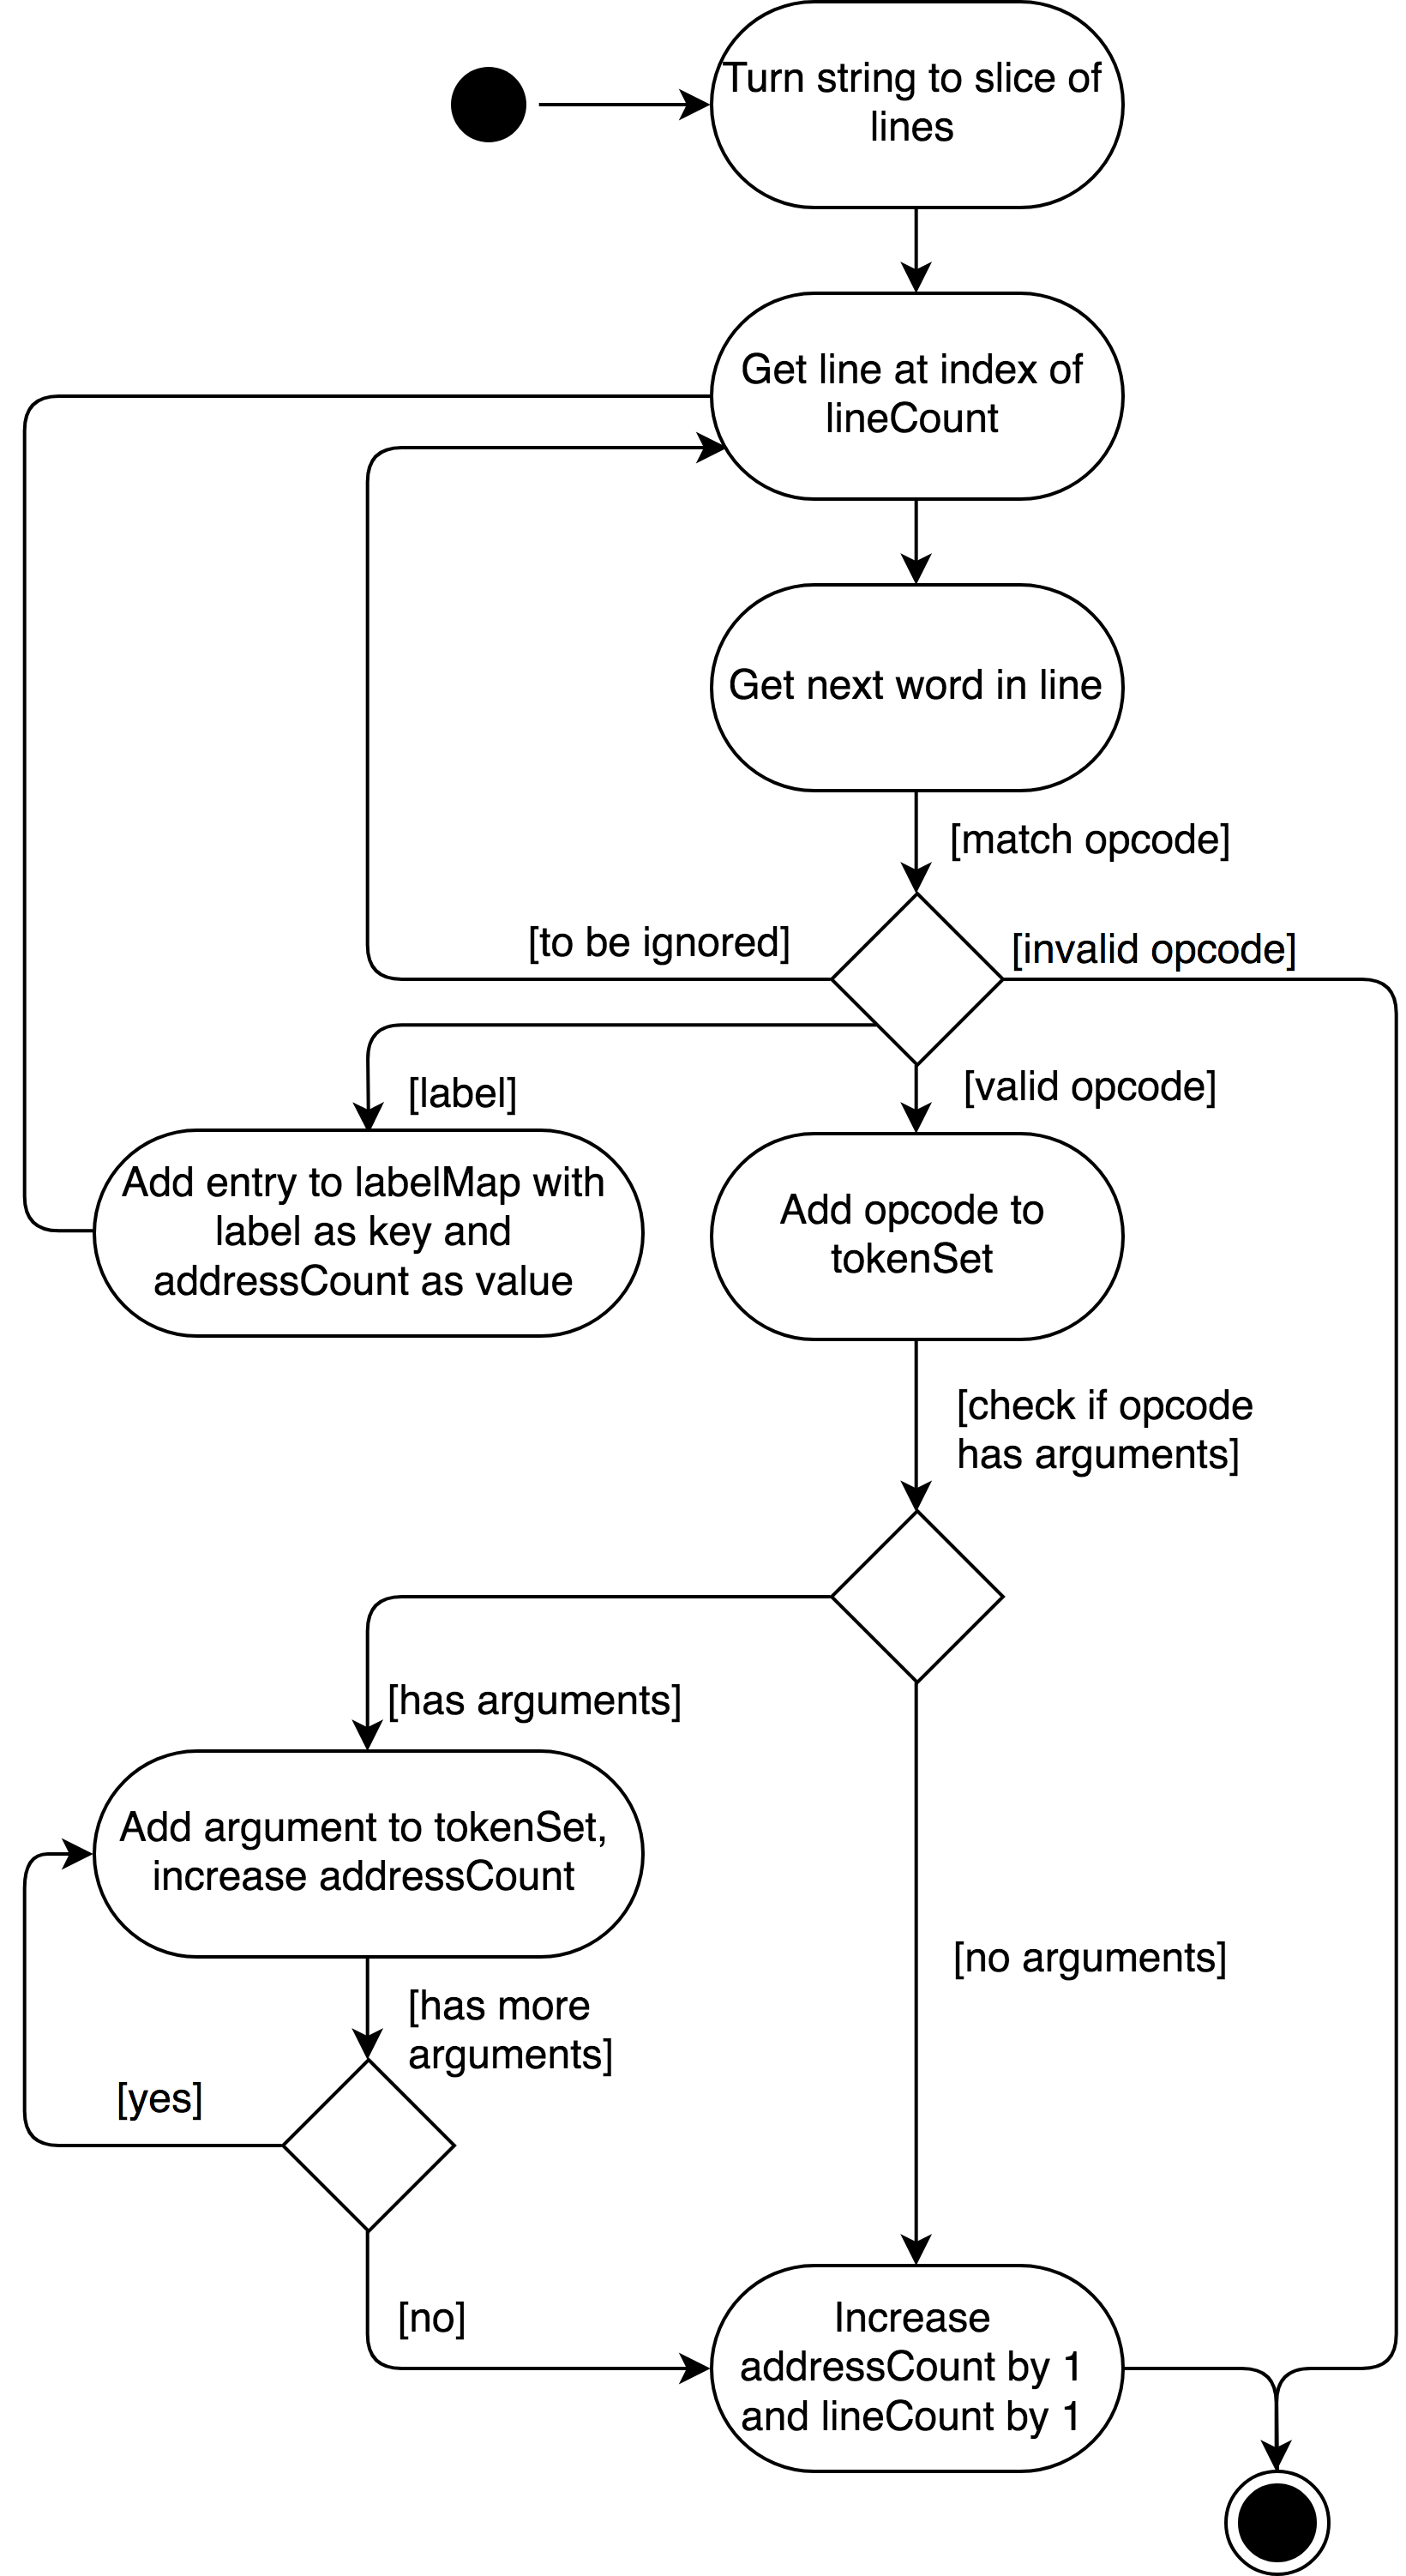
\includegraphics[width=0.5\textwidth]{./images/tokenize-function}
	\caption{UML Activity Diagram of the Tokenize Function}
	\label{tokenizefunc}
	\end{center}
\end{figure}

\begin{tabular}[t]{ p{3cm} p{12.5cm}}
\raggedright
\textbf{Token set} &
Code snippet \ref{tokenset} shows the generated token set to the basic contract shown in figure \ref{basiccontract_design} in the design chapter.
\end{tabular}

\begin{figure}[thp]%
    \centering
   	\begin{minipage}{0.4\textwidth}
\begin{minted}
[
	frame=lines,
	framesep=2mm,
	baselinestretch=1.2,
	fontsize=\footnotesize,
	linenos
]
{go}
{
[{0 PUSH} {1 55780}],
[{0 PUSH} {1 5}],
[{0 CALL} {4 addNums} {2 2}],
[{0 HALT}],
[{0 LOAD} {2 0}],
[{0 LOAD} {2 1}],
[{0 ADD}],
[{0 RET}],
}
\end{minted}
\end{minipage}
\caption{TokenSet of basic contract shown in \ref{basiccontract_design}}
\label{tokenset}
\end{figure}

\begin{tabular}[t]{ p{3cm} p{12.5cm}}
\raggedright
\textbf{Parse() function} &
The \mintinline{go}{Parse()} function compiles the token set to \flqq Bazo Byte Code\frqq. Figure \ref{parsefunc} shows the the process of the function. The function iterates over all tokens in the token set and matches the different types. If the type is \mintinline{go}{OPCODE} the matching byte value is added to the instruction set. If the type is \mintinline{go}{LABEL} the value is loaded from the labelMap, which is the jump address. A special type is \mintinline{go}{INT}. If an opcode takes an int value as an argument the first byte of the value shows the length of the byte representation. That means, that the byte representation of the value must be prepended with the amount of bytes the byte representation of the int requires. \mintinline{go}{BYTE} and \mintinline{go}{BYTES} just append the value to the instruction set. 
\end{tabular}

\begin{figure}[H]
	\begin{center}
	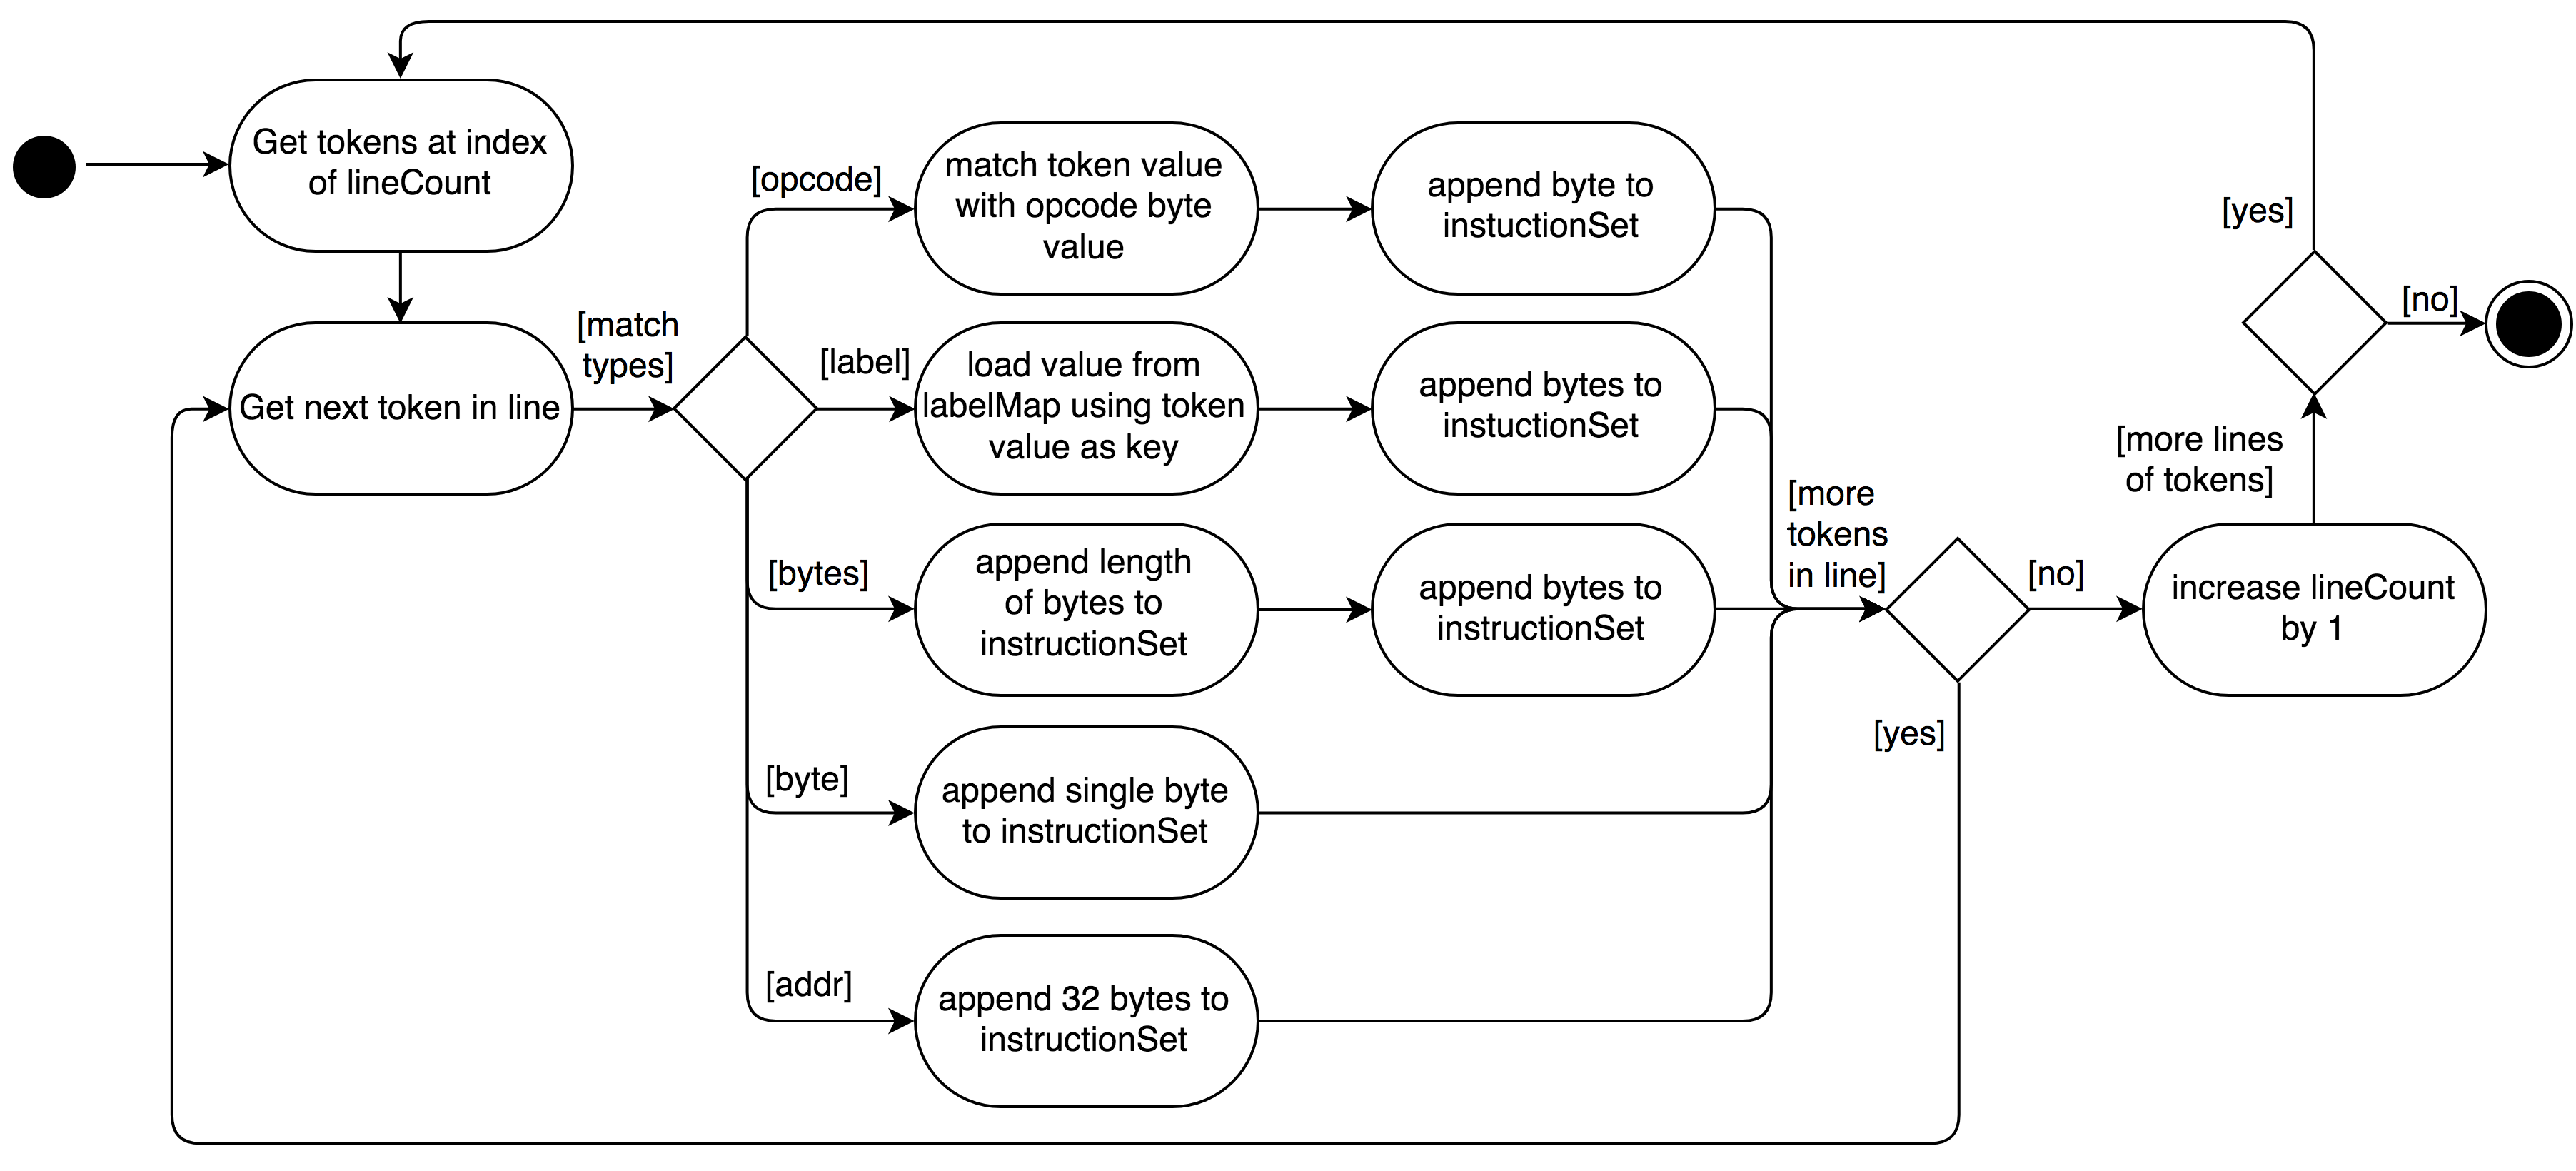
\includegraphics[width=\textwidth]{./images/parse-function}
	\caption{UML Activity Diagram of the Parse Function}
	\label{parsefunc}
	\end{center}
\end{figure}

\begin{tabular}[t]{ p{3cm} p{12.5cm}}
\raggedright
\textbf{Instruction set} &
Code snipped \ref{compiledbytecode} shows the resulting byte code instruction set.
\end{tabular}

\begin{figure}[thp]%
    \centering
   	\begin{minipage}{0.7\textwidth}
\begin{minted}
[
	frame=lines,
	framesep=2mm,
	baselinestretch=1.2,
	fontsize=\footnotesize,
	linenos
]
{go}
{
  0, 1, 217, 228, 0, 0, 5, 21, 0, 13, 2, 50, 28, 0, 28, 1, 4, 24, 
}
\end{minted}
\end{minipage}
\caption{Basic contract compiled to \flqq Bazo Byte Code\frqq}
\label{compiledbytecode}
\end{figure}

\section{Testing}
The virtual machine, the parser and integration were extensively tested from the start. Depending on the type of component and its relations, different testing methods have been applied. Overall a relatively high test coverage could be achieved. In the sections below, the different testing methods for each package are explained.

\subsection{Unit Testing}
All packages have been unit tested. Each modified package is compared with the package before integration to ensure that the test coverage is not negatively affected by the integration.

\begin{tabular}[t]{ p{3cm} p{12.5cm}}
\raggedright
\textbf{Protocol} &
As described in the sections before, not many changes have been made to the Protocol package. The test coverage before the VM integration was 70\%. The updated test coverage is 65\%, which shows, TODO  \\ \\
\textbf{Miner} &
The test coverage before the VM integration was TODO\%. The updated test coverage is TODO\%, which shows, TODO  \\ \\
\textbf{VM} &
The overall statement coverage is 81.7\%. Every component of the vm package has a test coverage over 78.8\%. The main component is the vm.go class. For every opcode at least one unit test has been made. Arithmetic opcodes are based on the big.Int implementation, which has been considered tested. This test coverage is influenced by the fuzz test described in Section \ref{fuzz_testing}. \\ \\
\textbf{Parser} &
The parser should be seen as a utility that is not part of the core project. For this reason, the necessity to test of this package was of low priority. Still a test coverage of 84.2\% could be achieved, because the package is small and the core class consists only of two main functions and a few helper methods. \\ \\
\end{tabular}
 
\subsection{Fuzz Testing} \label{fuzz_testing}
An instruction set of a smart contract must never be able to crash the miner. Calling a smart contract function with malicious instructions would cause the whole blockchain to collapse. To check if the VM fails gracefully, a fuzz test was implemented which creates contracts with real random bytes and then executes them. Contracts causing the miner to crash were reproduced as unit test in order to find the bug. Once the bug was found it was mitigated. This process was repeated over and over again. Starting the fuzz test with five million random contracts with every commit to the remote repository using Travis CI and having run it with a billion random contracts over night makes us confident that every bug that could crash the miner was found and mitigated. 

\subsection{Integration Testing}
To test whether the virtual machine could be successfully integrated, an integration test was made. The goal of this test is to show that deploying and calling smart contracts over transactions are possible. The integration test consists of multiple small unit tests. It was tested whether it is possible to create smart contract accounts, call functions of these smart contracts and whether state variables are persisted over several transactions.
%insert number of testcoverage
